\section{Implementación y Evaluación de la prueba de concepto}

Para el desarrollo de esta prueba de concepto, se ha pensado crear un smart contract que abarque todas las funcionalidades mencionadas en los apartados anteriores, y una interfaz web basada en pantallas, donde cada pantalla proveerá de la interoperabilidad necesaria para que el usuario pueda interactuar con el smart contract en la blockchain, y se le ha dado el nombre de \textit{UACrowdFunding} al sistema desarrollado.

\subsection{Implementaciones}

\subsubsection{Front-End ( Interfaz Web ) }

La aplicación de Front-End se ha desarrollado con Svelte como se ha mencionado en el apartado de Metodología. 

\bigskip

Se ha decidido desarrollar un Front-End realizando un sistema de tipo SPA, por su simpleza y fácil implementación con Svelte.

\bigskip

Las SPAs ( Single Page Application ) son páginas web que en vez de forzar al navegador cargar un archivo cada vez que se cambia de página dependiendo de la URL, estas ( mediante JavaScript ) reemplazan el contenido que está mostrando el navegador.

\bigskip

Esto da lugar a que la página web no se basará en URLS para navegar entre pantallas, sino que trabajará con estados, de tal forma que la página al cambiar de un estado a otro, esta rederizará un contenido HTML dinámico distinto. Los estados en los que se parte esta SPA son 6, una por cada pantalla de la interfaz: 

\bigskip

DESCONECTADO, CARTERA-INEXISTENTE, RED-EQUIVOCADA, LISTA-PROYECTOS, CREAR-PROYECTO, DETALLE-PROYECTO.

\bigskip

También cabe mencionar que la aplicación de Svelte usa de la librería EthersJS para conectarse con la cartera MetaMask embebida en el navegador, y así poder comunicarse con la red blockchain a través de la cuenta del usuario.

\newpage

A continuación se muestran las pantallas implementadas en el Front-End basadas en los Mockups.

\bigskip

\paragraph{Pantalla de Registro}
\begin{figure}[H]
        \centering
        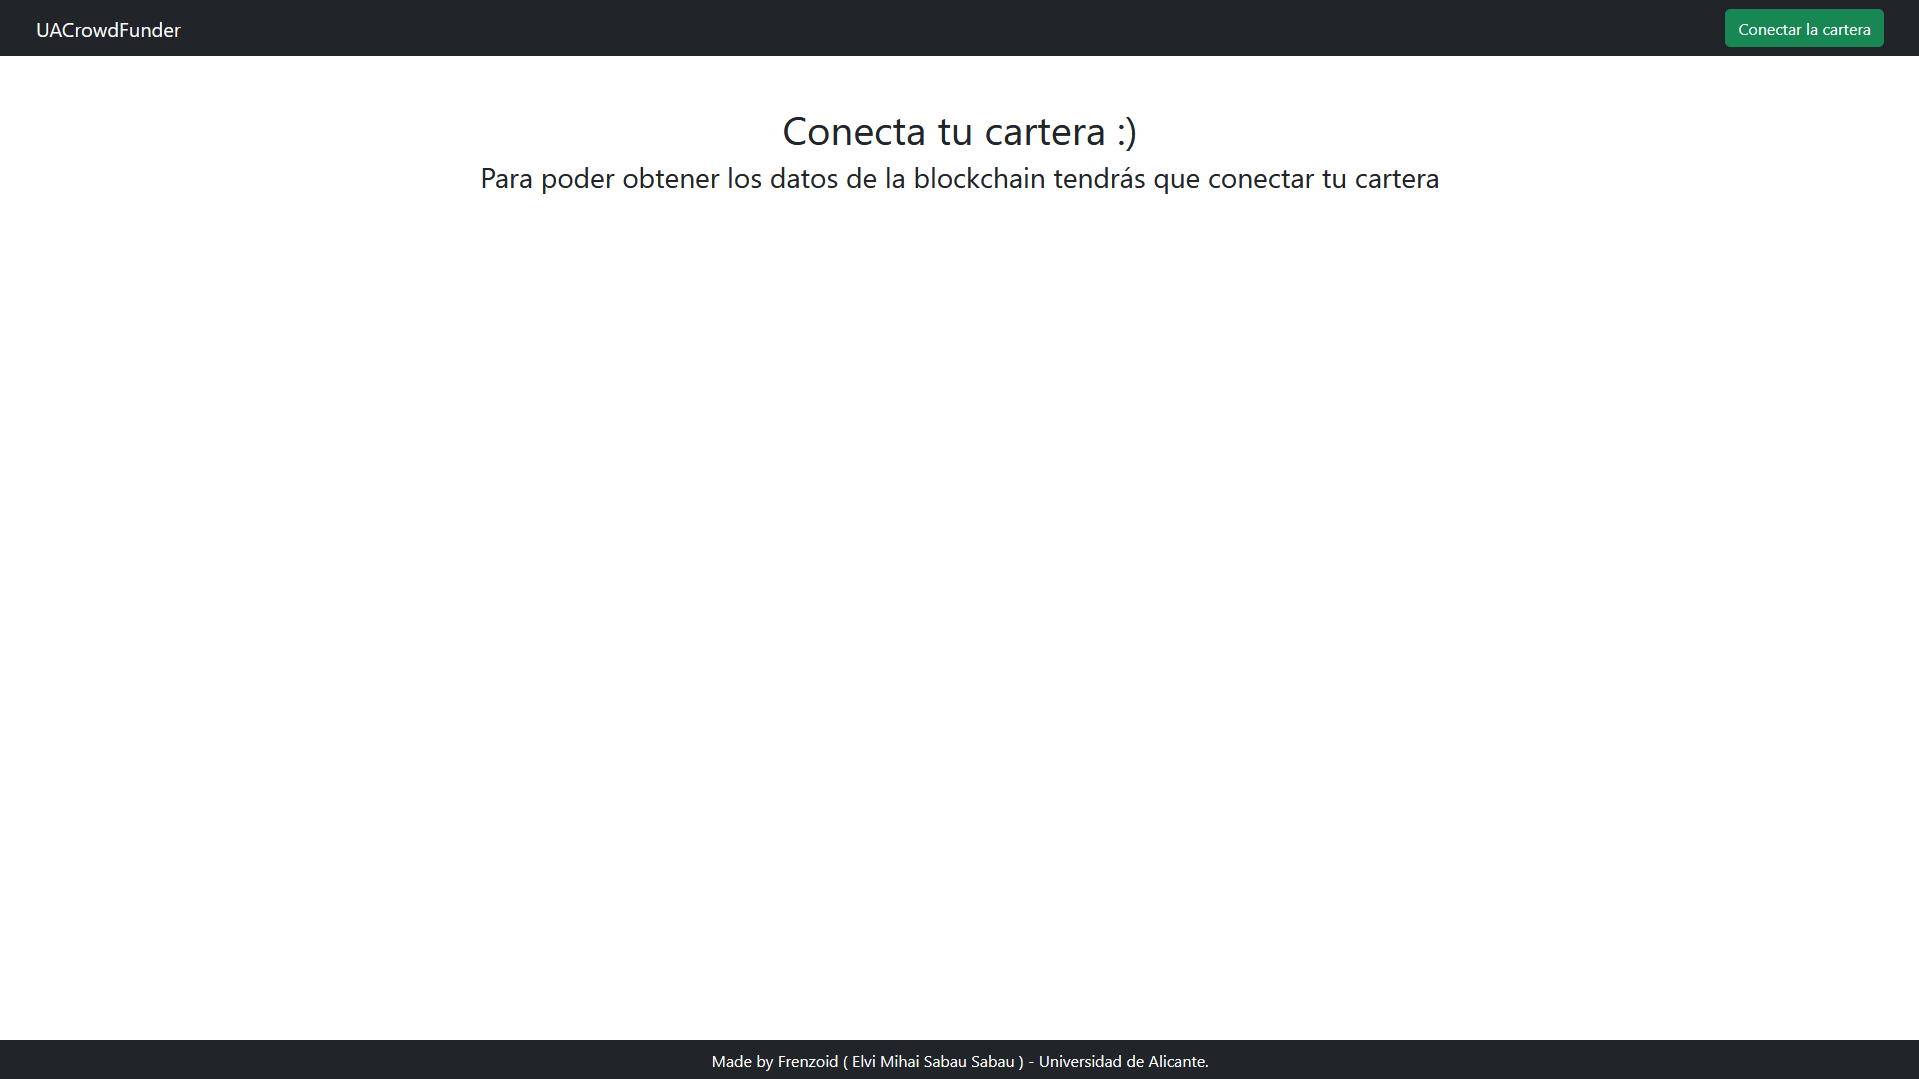
\includegraphics[width=1\textwidth]{img/interfaz/pantalla_registro.png}
        \caption{Interfaz Web - Pantalla de Registro.}
        \label{fig:configApi}
\end{figure}

\paragraph{Pantalla de notificación de red equivocada}
\begin{figure}[H]
        \centering
        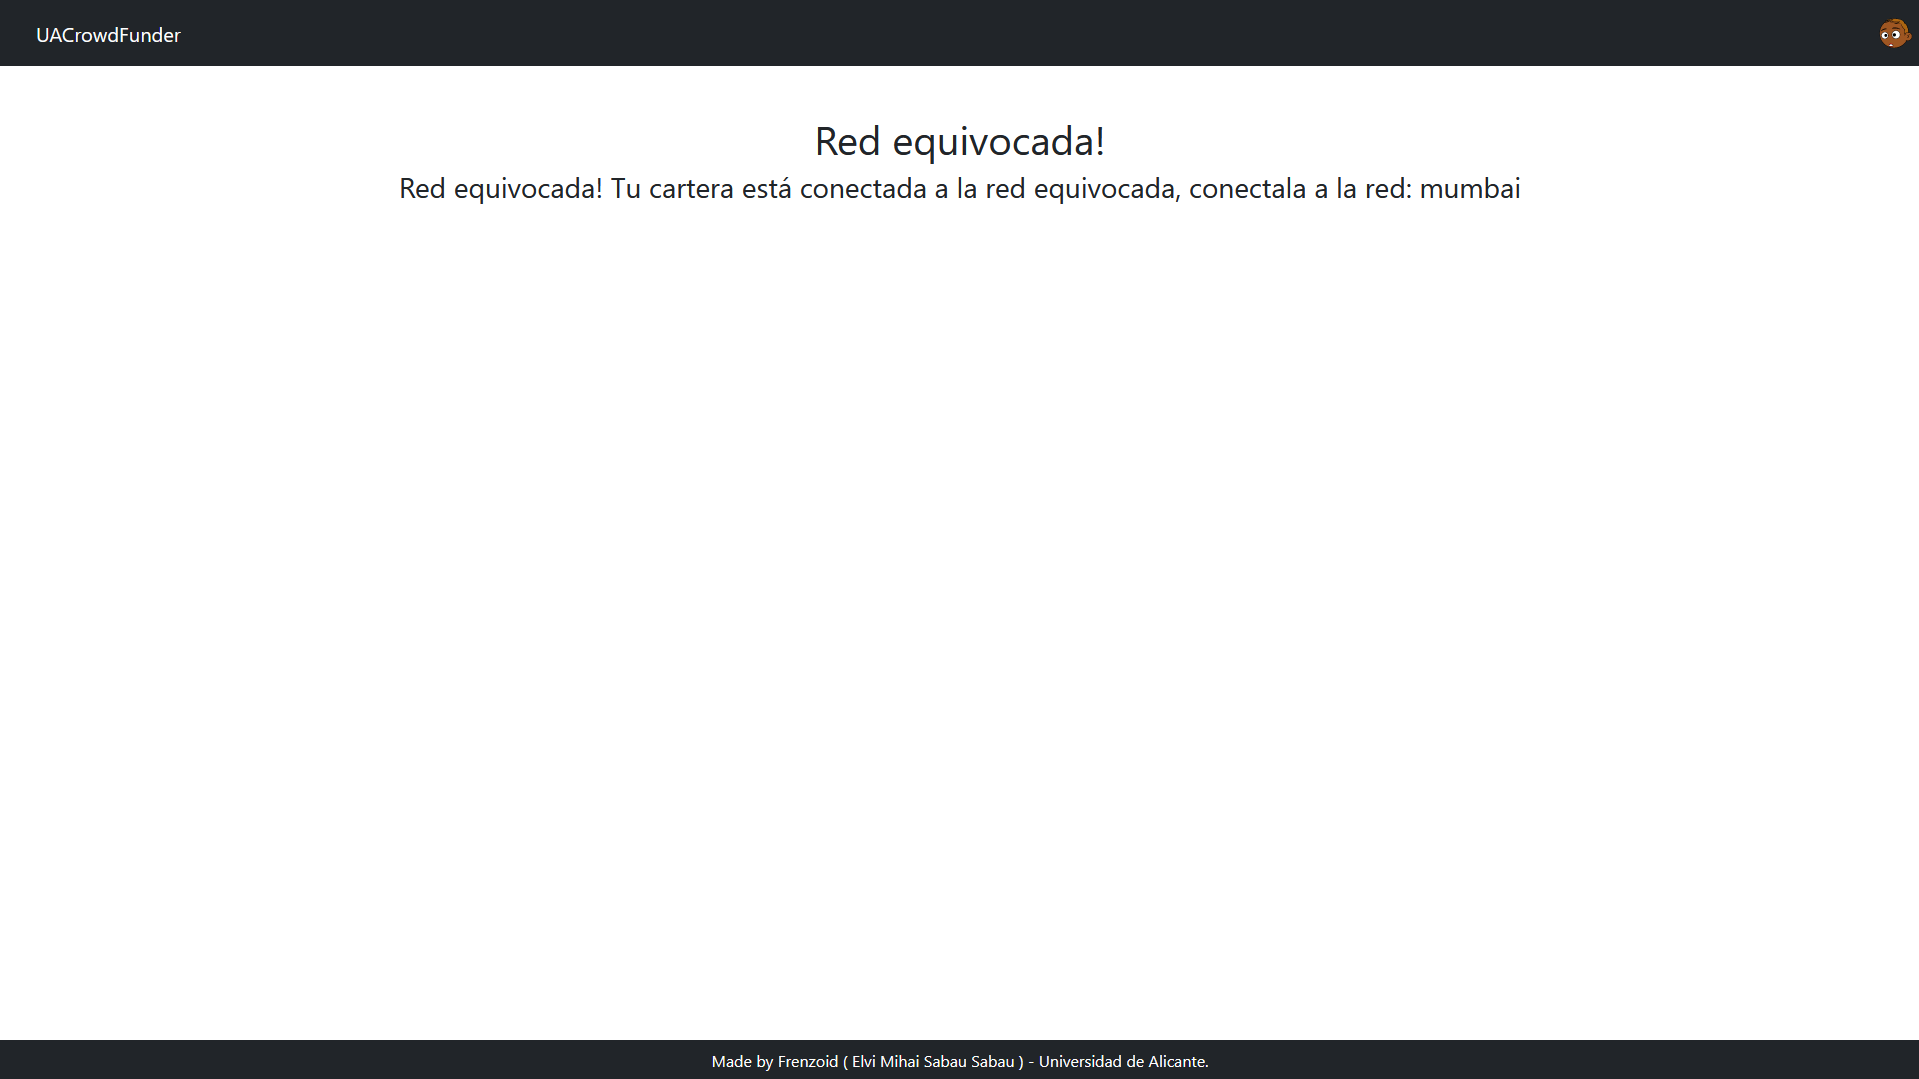
\includegraphics[width=1\textwidth]{img/interfaz/red_equivocada.png}
        \caption{Interfaz Web - Notificación de red equivocada.}
        \label{fig:configApi}
\end{figure}

\paragraph{Pantalla de notificación de cartera inexistente}
\begin{figure}[H]
        \centering
        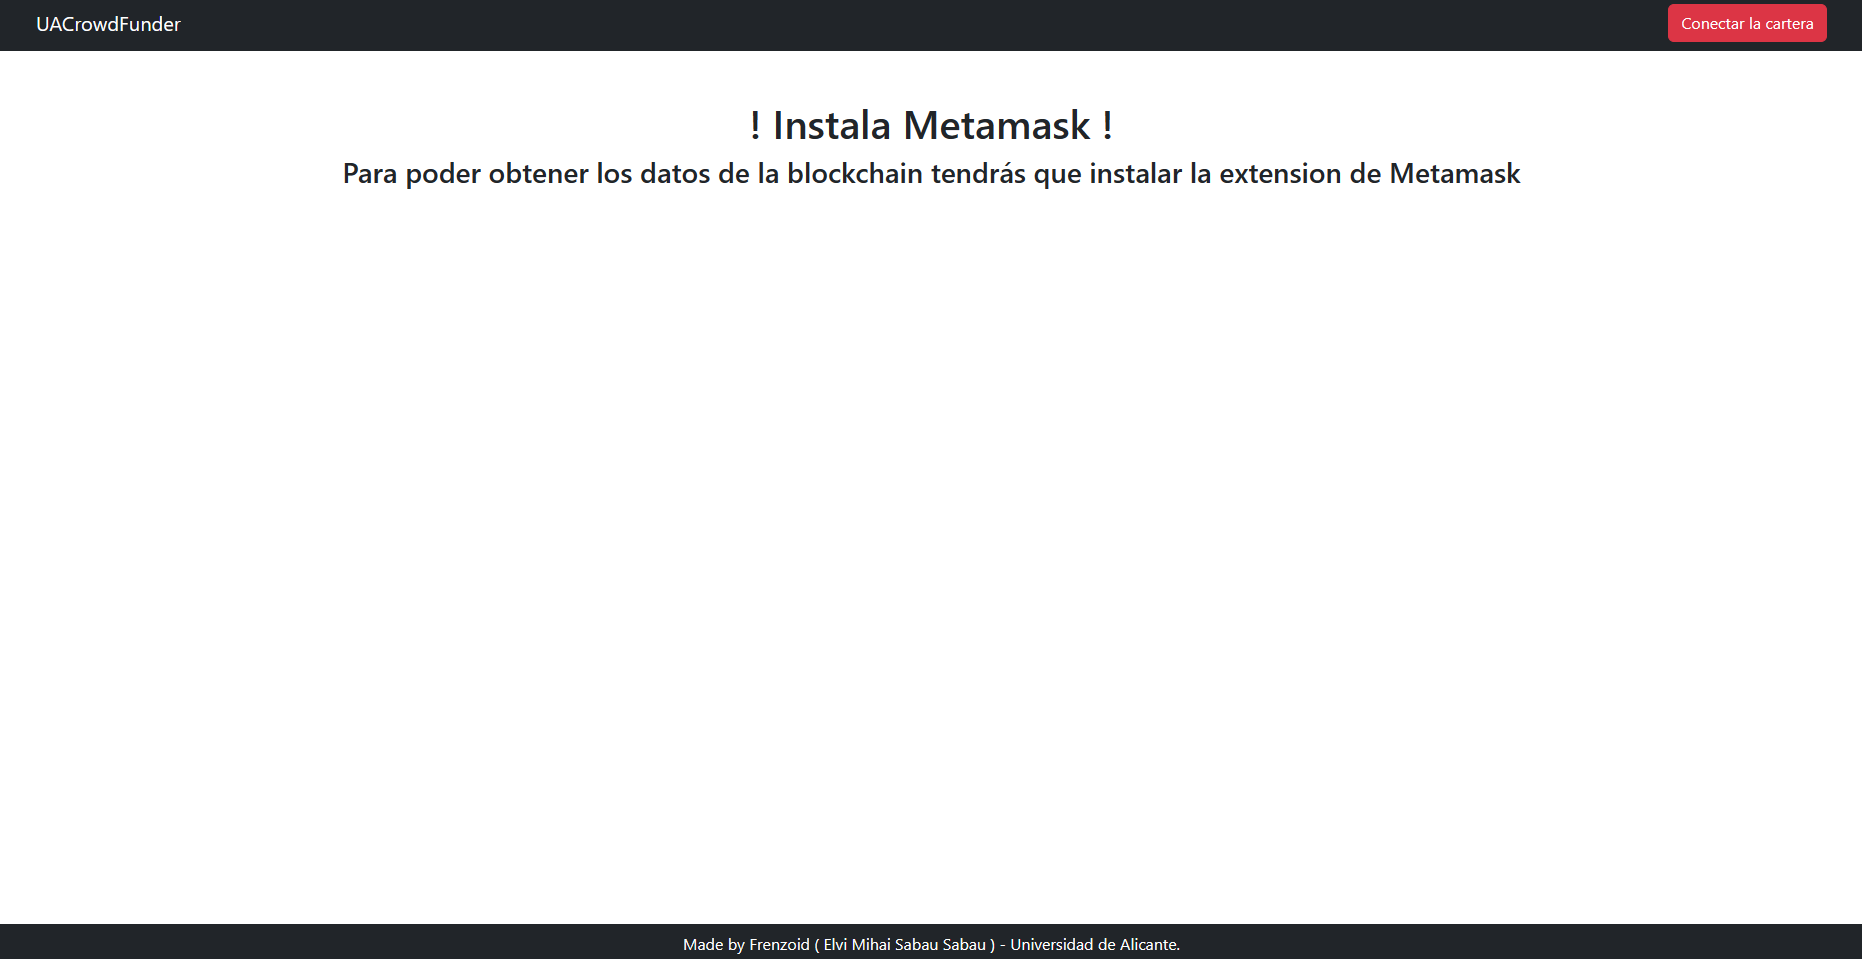
\includegraphics[width=1\textwidth]{img/interfaz/cartera_inexistente.png}
        \caption{Interfaz Web - Notificación de cartera inexistente.}
        \label{fig:configApi}
\end{figure}


\paragraph{Pantalla de la lista de Proyectos}
\begin{figure}[H]
        \centering
        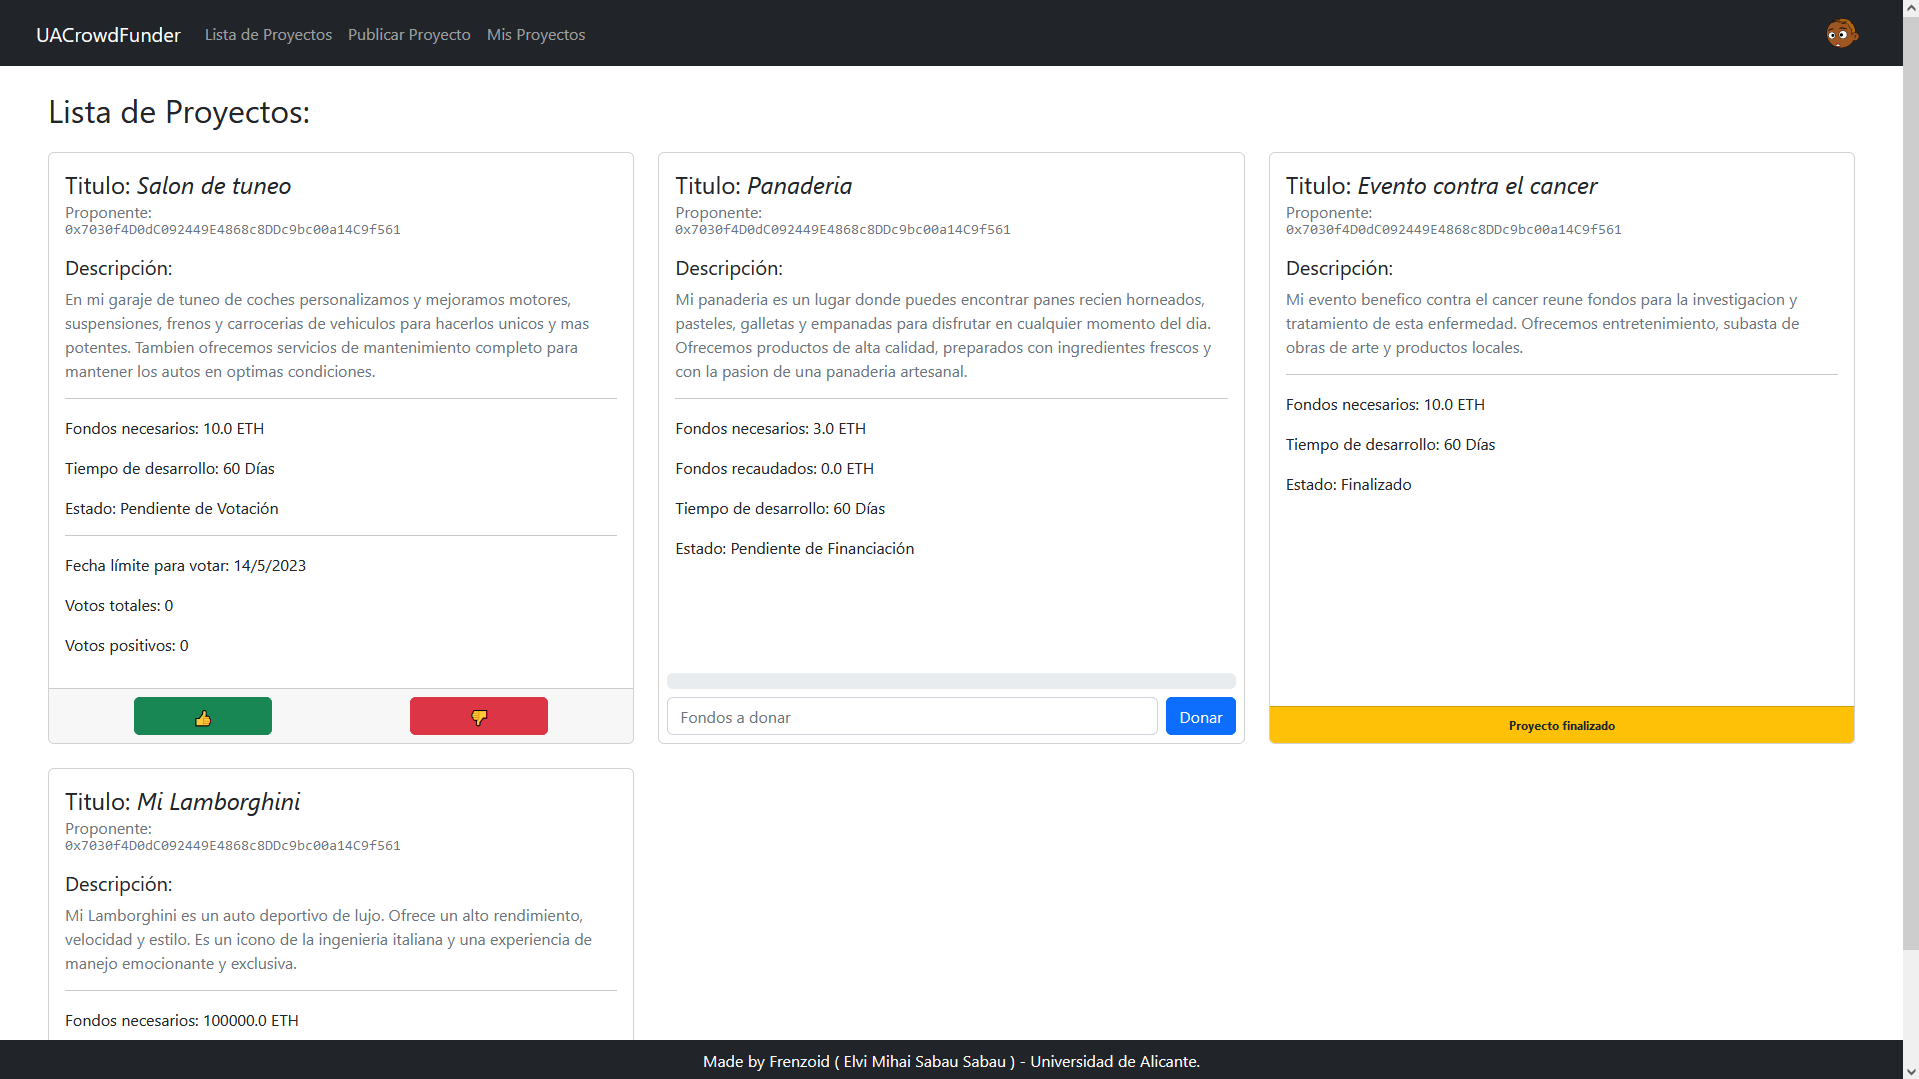
\includegraphics[width=1\textwidth]{img/interfaz/lista_proyectos.png}
        \caption{Interfaz Web - Lista de Proyectos.}
        \label{fig:configApi}
\end{figure}

\paragraph{Pantalla del formulario para proponer un proyecto}
\begin{figure}[H]
        \centering
        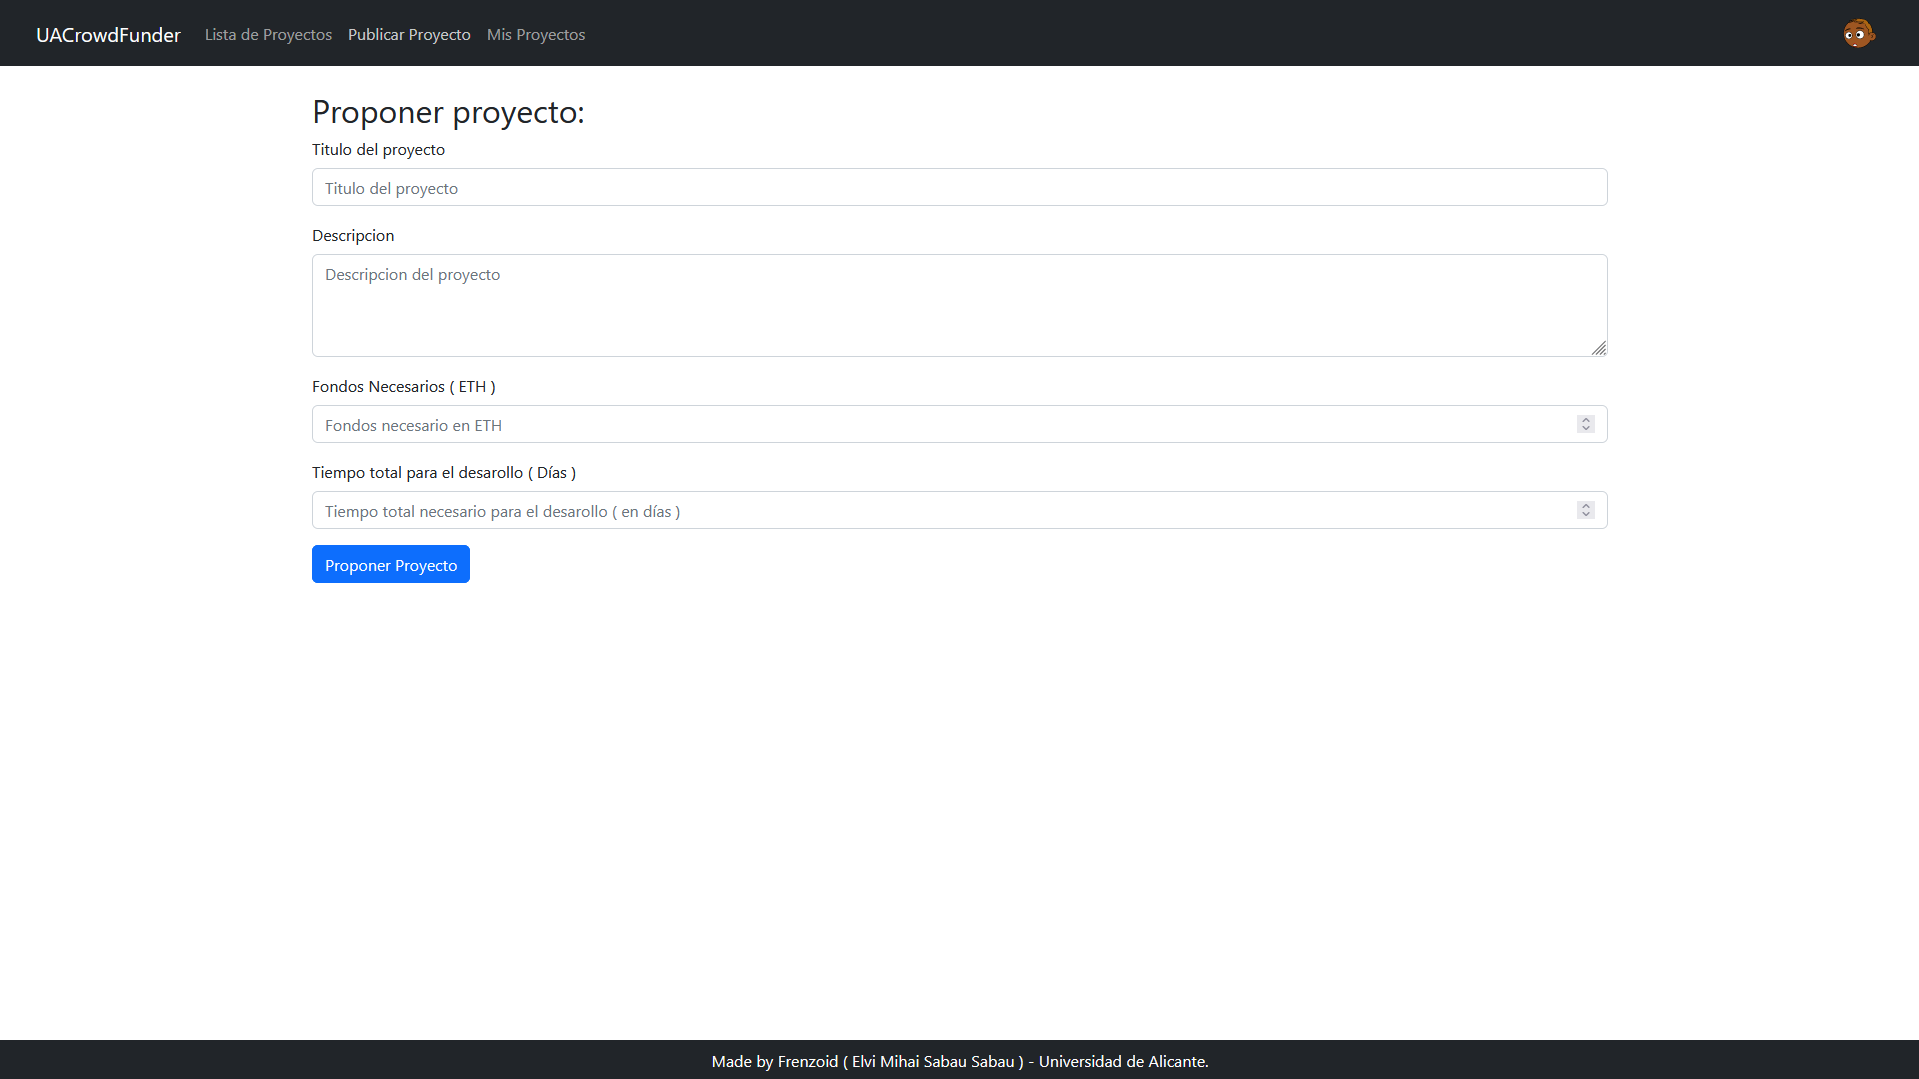
\includegraphics[width=1\textwidth]{img/interfaz/publicar_proyecto.png}
        \caption{Interfaz Web - Formulario para proponer un proyecto.}
        \label{fig:configApi}
\end{figure}

\paragraph{Pantalla de detalles de un proyecto}
\begin{figure}[H]
        \centering
        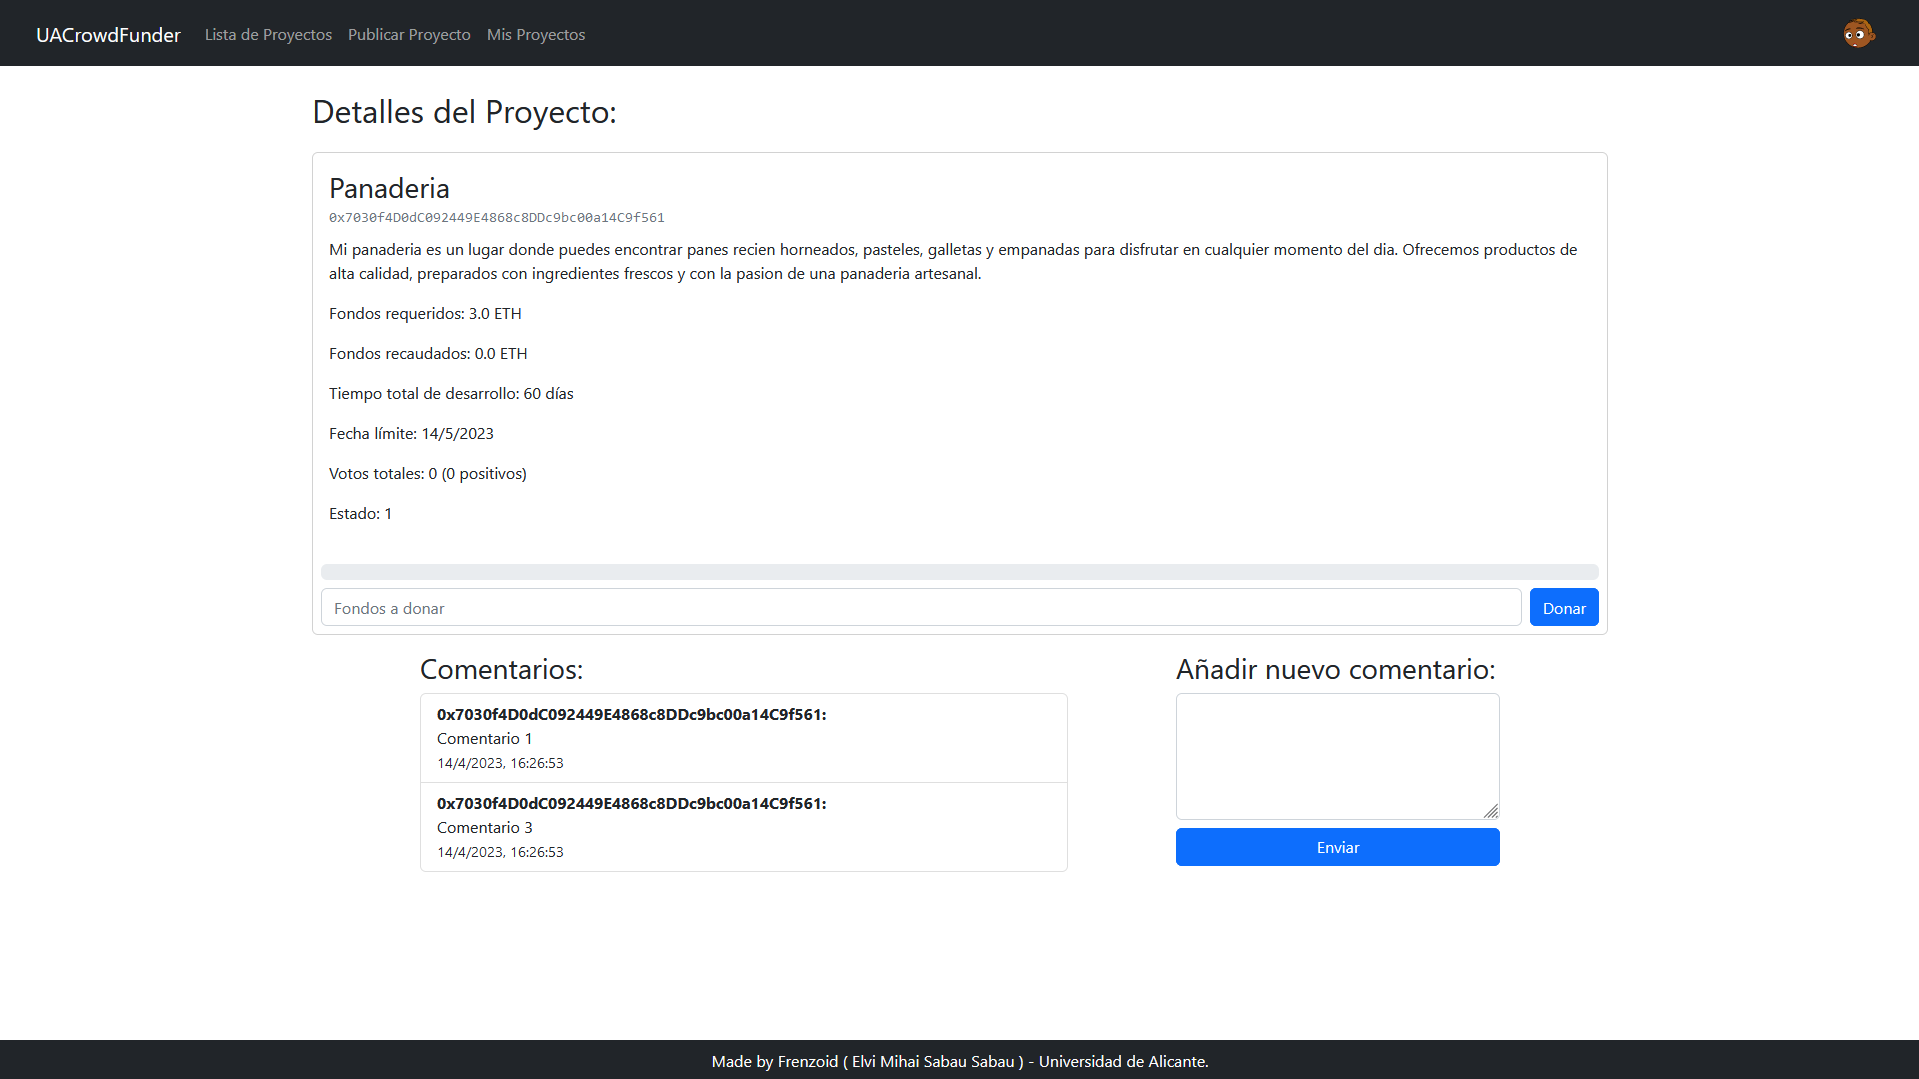
\includegraphics[width=1\textwidth]{img/interfaz/detalles_proyecto.png}
        \caption{Interfaz Web - Detalles de un proyecto.}
        \label{fig:configApi}
\end{figure}

Se ha tomado la decisión de alterar el diseño de la implementación de esta pantalla con respecto al mockup desarollado, para mostrar de forma más cómoda los comentarios y el formulario. 

\bigskip

La modificación que se ha realizado separa la lista de comentarios y la funcionalidad de enviar un nuevo comentario en 2 columnas separadas.

\newpage

\subsubsection{Back-End  ( DAO ) }
El smart contract que se desarrolla deberá implementar las variables y funciones de la interfaz mencionada en el capitulo anterior (Capitulo 6.4.3).

\bigskip

Este implementará las funcionalidades necesarias para el desarrollo de la prueba de concepto, incluyendo los objetos necesarios para gestionar proyectos, comentarios, gestión de fondos, etc.

\bigskip

\textit{NOTA: Para agilizar la presentación de la prueba de concepto, se ha decidido agregar 4 propuestas de ejemplo desde el constructor del smart contract.}

\bigskip

\paragraph{Implementación del Smart Contract}

A continuación se muestra el código fuente del smart contract implementado.

\bigskip

\lstinputlisting[language=Solidity, caption=Smart Contract de la prueba de concepto.]{codigo/contratos/ProjectPlatformDemo.sol}

\newpage

\subsection{Despliegue del sistema}

\subsubsection{Código fuente del proyecto}

El código del proyecto se encuentra en la siguiente \textcolor{blue}{\href{https://github.com/Frenzoid/UA_TFG}{\textbf{dirección}}}, para arrancarlo solo se debe seguir los pasos descritos en los archivos \quotes{README} de ambas carpetas ( Front-End y Back-End ).

\bigskip

Para el despliegue de este sistema usaremos diferentes herramientas que se han mencionado en el contexto tecnológico.

\subsubsection{Despliegue de la interfaz web}

Para desplegar la aplicación de Svelte usaremos Docker. Docker, como ya se ha explicado en apartados anteriores, es una plataforma que sirve para encapsular servicios en contenedores, y desplegarlos en cualquier máquina que ejecute Docker.

\bigskip

De esta forma, el servicio a desarrollar se vuelve portable, y se aísla tanto en recursos como en configuración del esto de servicios ejecutándose en el servidor.

\bigskip

\paragraph{Sobre la metodología del despliegue}

Tal como se menciona en el capítulo de Metodología, se propone un despliegue con CI mediante Github Actions y utilizando DockerHub para automatizar dicho despliegue. Sin embargo, en esta sección se detalla un despliegue manual con el objetivo de explicar en profundidad este proceso, abordando las partes que conforman Docker y el despliegue de la aplicación en un contenedor.

\bigskip

Así que, en este caso la aplicación se despliega en un VPS\footnote{VPS: Servidor Virtual Privado.} con Docker instalado, de esta forma tendremos el la aplicación de Svelte ejecutándose en un contenedor en el VPS las 24hrs del día.
\paragraph{Encapsulando la aplicación web}

Para generar un contenedor desde la app de Svelte, primero vamos a necesitar generar una \quotes{imagen} de la aplicación. Una imagen es el conjunto de archivos y comandos que contendrá y ejecutará un contenedor, muy similar a una ISO, pero en Docker.

\newpage

Para generar una imagen, lo único que se necesita es declarar en un archivo llamado \quotes{Dockerfile} los archivos a encapsular en la imagen, los comandos necesarios para preparar la aplicación, y por ultimo el comando que se ejecutará dentro del contenedor para desplegar el servidor web.

\bigskip

A continuación se muestra el Dockerfile.

\bigskip

\begin{figure}[H]
        \centering
        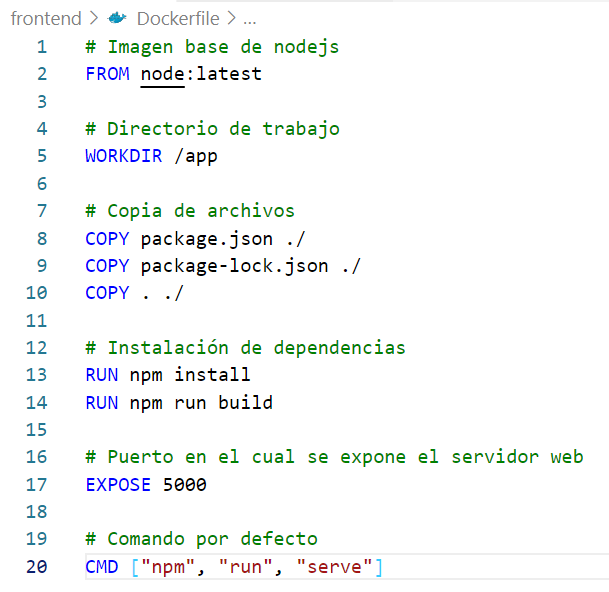
\includegraphics[width=0.7\textwidth]{img/capturas/Dockerfile.png}
        \caption{Dockerfile - Dockerfile del Front-End.}
        \label{fig:configApi}
\end{figure}

\bigskip

Para generar la imagen se ejecuta el comando: \quotes{docker build . -t elvi/tfg:latest}. El nombre de la imagen se asigna con el parámetro -t, y la nomenclatura del nombre es  \quotes{autor}/\quotes{servicio}:\quotes{versión}.

\bigskip

Mediante docker se publica la imagen a DockerHub, un repositorio de imágenes de Docker, y una vez publicado es posible arrancar el Front-End desarrollado en cualquier ordenador que tenga docker instalado.

\bigskip

Para arrancar un contenedor con la imagen se ejecuta el siguiente comando: \quotes{docker run --name \quotes{FRONTEND\_TFG} -p 5000:5000 elvi/tfg:latest}.

\bigskip

El parametro -p indica el mapeo de puertos del \quotes{anfritrion}:\quotes{contenedor}.

\begin{figure}[H]
        \centering
        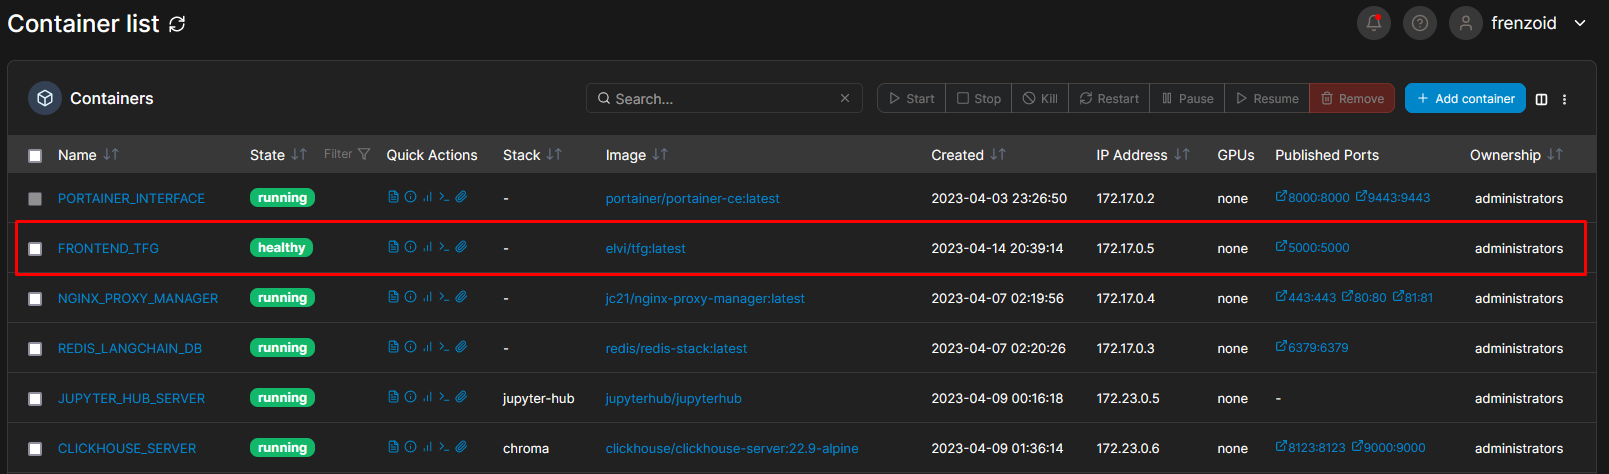
\includegraphics[width=1\textwidth]{img/capturas/portainertfg.png}
        \caption{Portainer - Interfaz de Portainer, gestor de contenedores de Docker.}
        \label{fig:configApi}
\end{figure}

En el VPS, mediante Portainer, se tiene la posibilidad de gestionar los contenedores desplegados. Al acceder al dominio o dirección IP del VPS seguido de :5000 \footnote{5000 es el puerto en el que la aplicación web permanece a la espera de conexiones.}, se puede visualizar la aplicación de Svelte que ha sido desplegada en el servidor.


\begin{figure}[H]
        \centering
        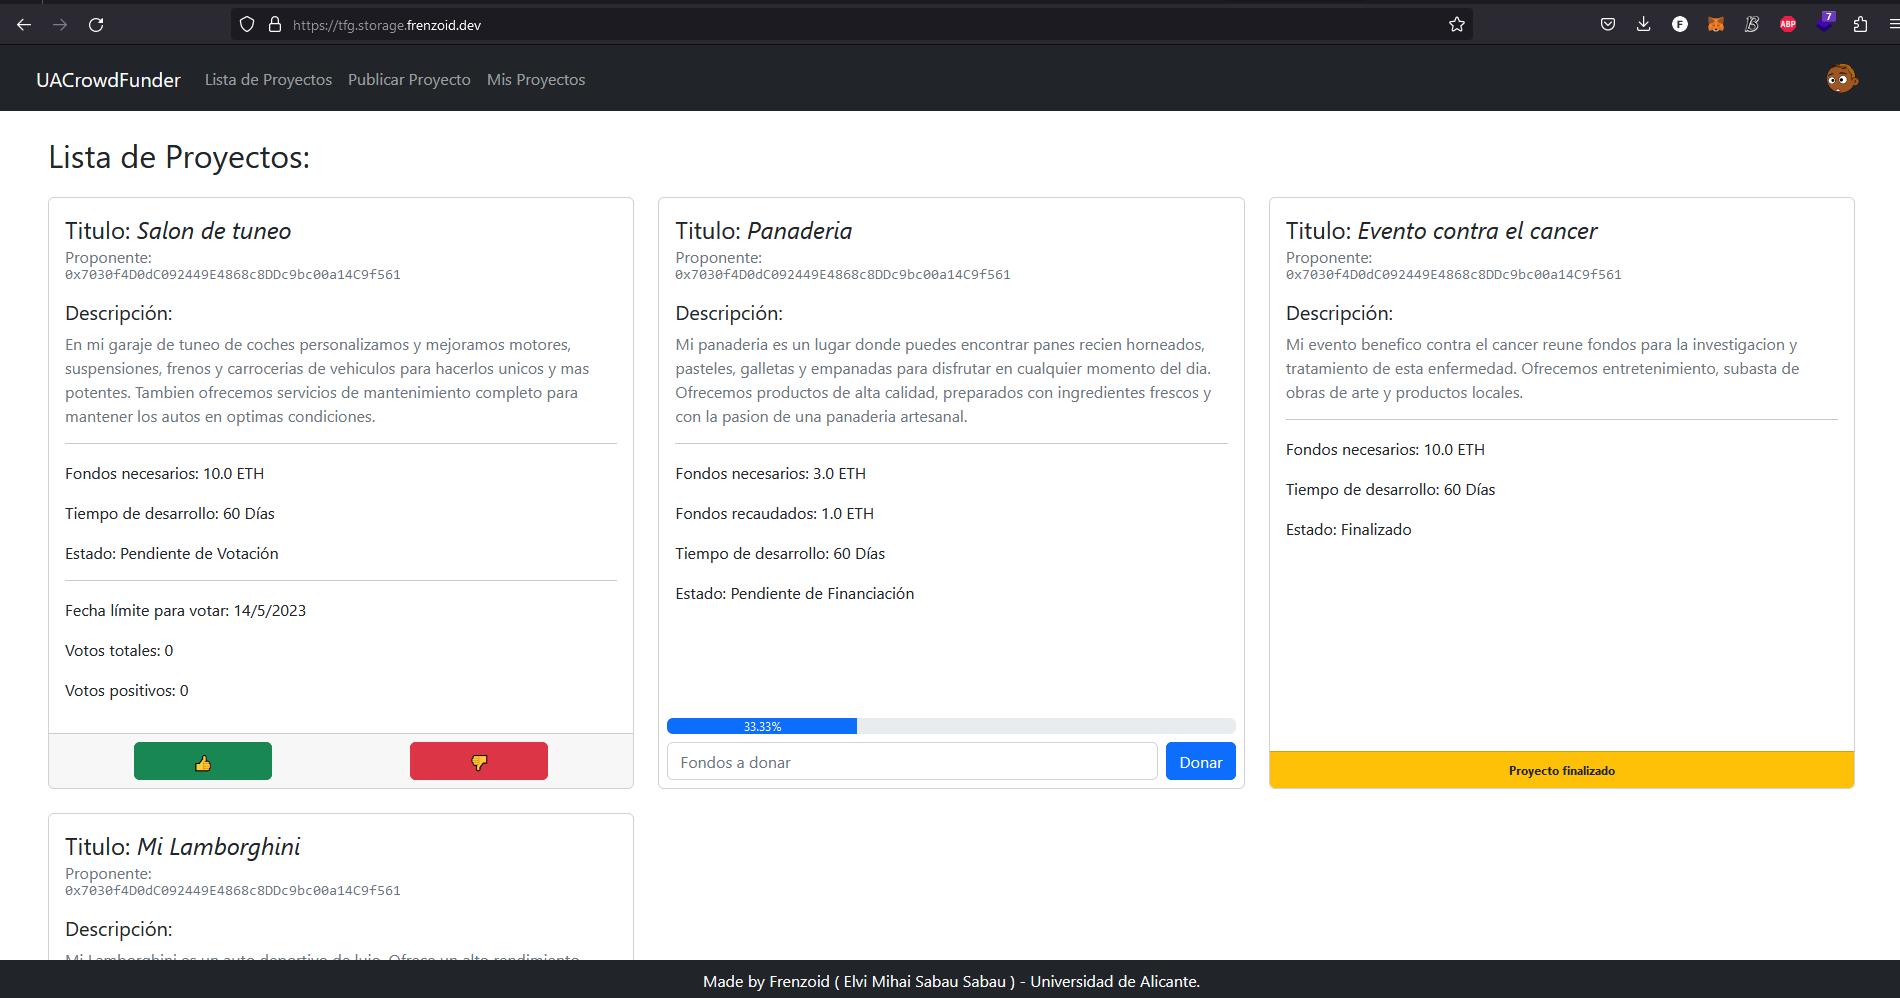
\includegraphics[width=1\textwidth]{img/capturas/frontendtfg.png}
        \caption{Front-End - Muestra de la aplicación desplegada.}
        \label{fig:configApi}
\end{figure}

El Front-End ahora está desplegado en la siguiente dirección: \textbf{https://tfg.storage.frenzoid.dev/}

\newpage

\subsubsection{Despliegue del Smart Contract}

El despliegue del smart contract se realizará mediante la herramienta HardHat, que posibilita la compilación, el despliegue y la validación de un contrato en cualquier red blockchain basada en el protocolo Ethereum.

\bigskip

A través de una plantilla\footnote{https://github.com/Frenzoid/DAPP\_DevKit\_1} que desarrollé, el despliegue de los contratos se automatiza, siendo sólo necesario especificar en el comando de despliegue la red donde se desea desplegar el contrato. Dicho comando se ejecuta en la carpeta \quotes{Back-End}, y presenta la siguiente sintaxis: \quotes{npm run deploy-RED}.

\bigskip

En el escenario de este proyecto, el contrato se despliega en la red de pruebas "Mumbai" de Polygon, por lo que la cuenta utilizada para desplegar el contrato necesitará disponer de MATIC, la criptomoneda de la red de Polygon.

\bigskip

La obtención de MATIC en la red de prueba puede llevarse a cabo utilizando las \textcolor{blue}{\href{https://mumbaifaucet.com/}{\textbf{faucets públicas de Mumbai}}}, con el objetivo de conseguir suficiente MATIC para cubrir los costes de desplegar el contrato en la red de prueba. Una vez adquirido un cierto volumen de MATIC, es posible proceder con el despliegue del contrato usando HardHat. Para ello, simplemente se necesita ejecutar el comando \quotes{npm run deploy-mumbai} en la carpeta \quotes{Back-End} del proyecto.

\bigskip

Al ejecutar este comando, HardHat revisará el código notificando cualquier error encontrado durante la compilación, empaquetará el contrato y exportará 2 archivos: el binario del contrato que se cargará en la blockchain, y una interfaz del contrato que se usará por la librería Ethers del Front-End para poder comunicarse con el contrato.

\bigskip

Una vez que el contrato es cargado y minado en la red, HardHat procederá automáticamente a validar el contrato, subiendo el código fuente del contrato a la red, de esta manera, se hacen públicas las funcionalidades del contrato a través de los exploradores de bloques como Polyscan.

\begin{figure}[H]
        \centering
        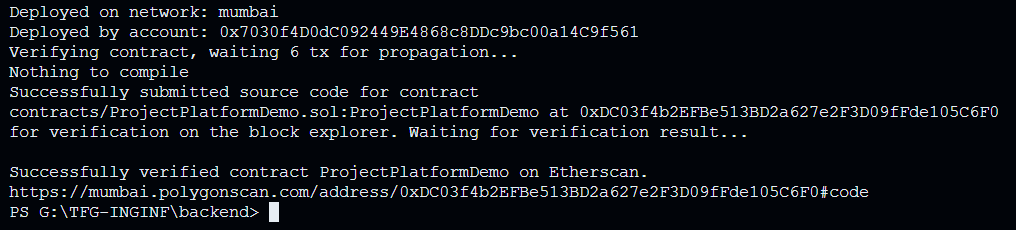
\includegraphics[width=1\textwidth]{img/capturas/validated.png}
        \caption{Verificación del contracto - Captura de la terminal, HardHat notificando de la correcta validación del contrato en la red Mumbai.}
        \label{fig:configApi}
\end{figure}

\textit{NOTA: La dirección del contrato que se muestra en la captura es diferente debido a que se desplegó múltiples veces durante la realización de este documento.}

\bigskip

Validar un contrato inteligente sirve para verificar y asegurar la transparencia del código fuente de dicho contrato en la red. Polyscan permite a los usuarios examinar el contrato en busca de posibles vulnerabilidades, errores o actividades sospechosas antes de interactuar con él.

\newpage

\paragraph{Verificación del contrato}

Una vez desplegado el contrato en la red de Mumbai, se puede presenciar el contrato desde el explorador de bloques de Polygon denominado Polyscan, y validar que se ha verificado el código fuente correctamente.

\begin{figure}[H]
        \centering
        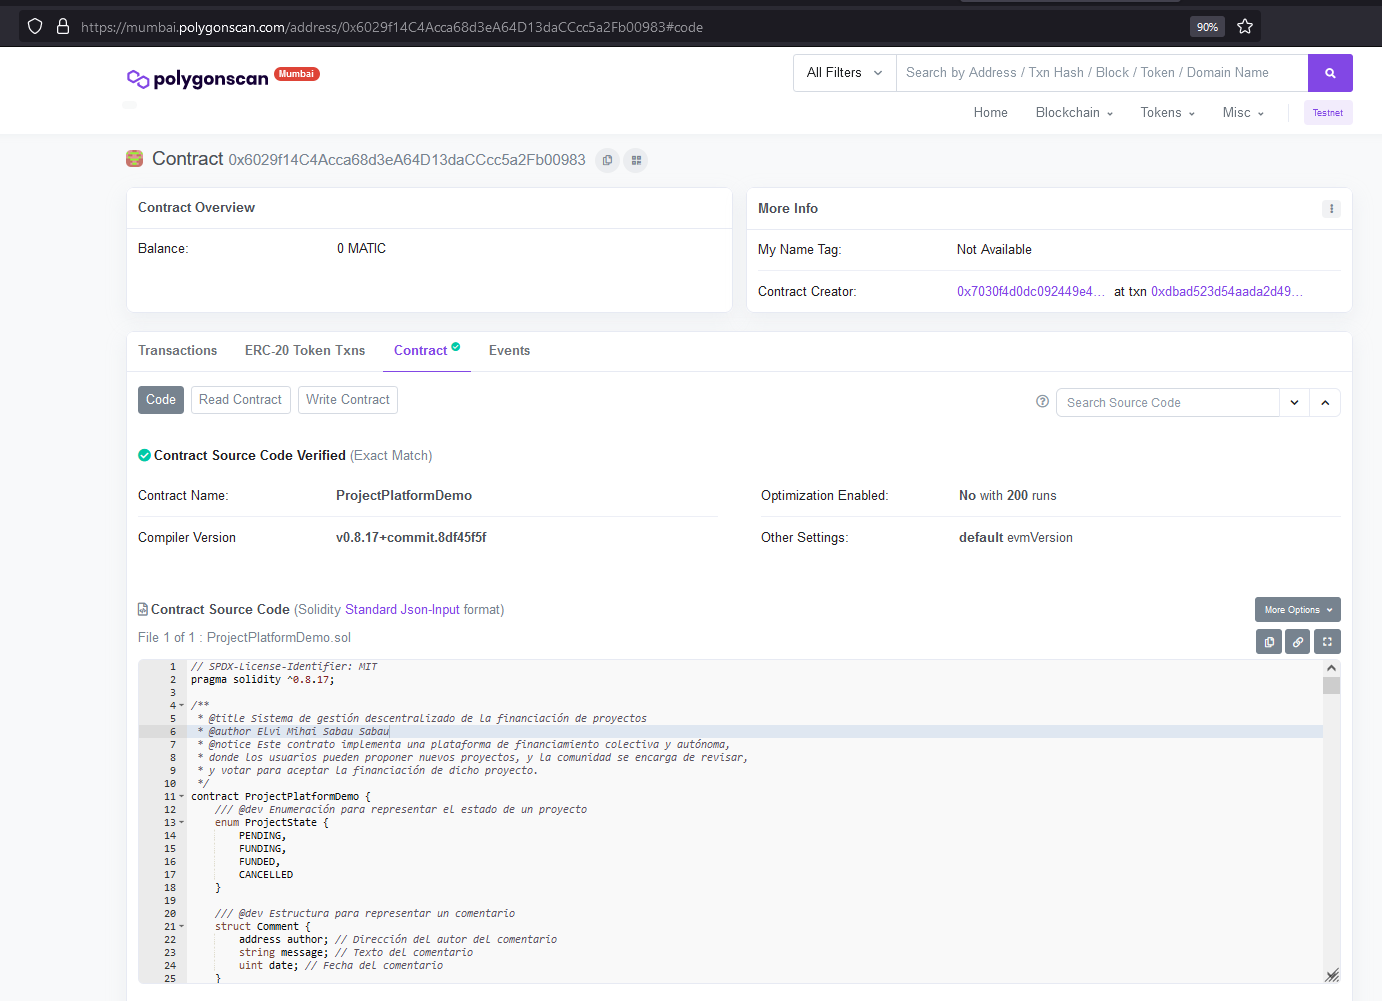
\includegraphics[width=1\textwidth]{img/capturas/etherscan.png}
        \caption{Polyscan - Captura del contrato desplegado y verificado en la red de Mumbai.}
        \label{fig:configApi}
\end{figure}

Se puede observar el contrato que se usará para la demostración en esta dirección:

\bigskip
\begin{center}
    \textbf{https://mumbai.polygonscan.com/address/0xE29548B54a978eeb4d071e6D7bd83871b2d56CAE}
\end{center}

\newpage

\subsection{Evaluación de la prueba de concepto}

En el siguiente enlace se muestra un vídeo de la prueba de concepto desarrollada, donde se explica cada pantalla y se demuestra su funcionalidad. El objetivo de este vídeo es validar la viabilidad del sistema desarrollado de la solución propuesta.

\bigskip

\begin{center}
    \textbf{https://youtu.be/DrpZKpXmicU}
\end{center}